\documentclass[conference]{IEEEtran}
% If the IEEEtran.cls has not been installed into the LaTeX system files,
% manually specify the path to it.  e.g.
% \documentclass[conference]{./IEEEtran}

% Add and required packages here
\usepackage{graphicx,times,amsmath, fontenc, epstopdf}
\usepackage[utf8]{inputenc}
\usepackage[T1]{fontenc}
\usepackage{hyperref}
\usepackage{listings}



% Correct bad hyphenation here
\hyphenation{op-tical net-works semi-conduc-tor IEEEtran}

% To create the author's affliation portion using \thanks
\IEEEoverridecommandlockouts

\textwidth 178mm
\textheight 239mm
\oddsidemargin -7mm
\evensidemargin -7mm
\topmargin -6mm
\columnsep 5mm

\begin{document}
	
	\lstset{basicstyle=\ttfamily, frame=shadowbox}

% Paper title: keep the \ \\ \LARGE\bf in it to leave enough margin.
\title{\ \\ \LARGE\bf Combining Clustering and Grammars \\ for Adaptive Level Generation\thanks{Jorge Diz and David Camacho are with the Computer Science Department, Escuela Politécnica Superior, Universidad Autónoma de Madrid. c/ Francisco Tomás y Valiente 11, 28049 Madrid, Spain. (email: {\tt jorge.diz@estudiante.uam.es} and {\tt david.camacho@uam.es})}}

\author{Jorge Diz Pico, David Camacho}

% Uncomment out the following line for invited papers
%\specialpapernotice{(Invited Paper)}

% Make the title area
\maketitle

\begin{abstract}
	
	Procedural content generation has been widely used to expand games
	of very diverse genres. Creating levels on the fly offers a fresh
	take on every run and infinite replayability. Adaptive techniques,
	on the other hand, strive to make this generation tailored to the user
	preferences, needs or skills. This paper offers a new take at
	an architecture that implements both by combining clustering
	for player profiling and grammars for defining level structure.
	Levels are created by traversing the derivation tree and
	generating a unique trace of level parts that can be
	used for identifying and comparing them. The system has
	been developed and tested for the Mario AI Championship competition,
	making use of their experimental platform.

\end{abstract}

% No keywords



\section{Introduction}

In the first years of the game industry, disk space was severely limited. A game's length was primarilly constrained by its size in bytes. In the 1980s, when home computing started to rise \cite{shah05}, the main shipping mediums were floppy disks or casettes (both around 1.2 MB). That put a cap on the amount of different playing levels a game could contain. But the design effort also played a big part. A game that wanted to ship with many different levels needed each of them carefully crafted and balanced by the gamemakers, taking a big chunk of the budget because of the time and money involved. The game industry was still in its infancy, with many of the titles being developed by only one person \cite{discovery}, and couldn't afford all that investment.

To solve this problem, early games started to develop algorithms to create levels in a procedural way. That is, creating a set of rules to build game levels on the fly, with a random component, ensuring  giving birth to procedural content generation. The most classic example is \textit{Rogue} \cite{rogue}, a roleplaying adventure game where the dungeons are generated at the beginning of each game. The influence of its style spawned a new genre of games called roguelike \cite{roguelike}.

Even if the disk space limitations are no longer present today, PCG techniques offered other clear advantages that made it be still in use today. The main feature that make procedural algorithms quite appealing for voth developers and players is its guarantee of infinite replayability. A game with a fixed array of levels to play has also a fixed (although possibly quite long) life length. It can be feasible to reach the end of its available possibilities. A game that offers a new, unique level everytime it is run, is virtually unfinishable \cite{rodenparberry2004}. Developers can create more experiences with not a bigger effort, and players get longer enjoyment for the same price. Examples can be found in all genres, from adventures \cite{diablo} and strategy \cite{civilization} to sandbox-building \cite{minecraft}.

Having rules in place to create levels can also help prepare the game for unexpected situations. For example, in a strategy game, it could be interesting to explore the dynamics of having less resources on the map. A player may even enjoy this increase in the effective power of the military in securing these resources. But most groundbreaking was the realization that since PCG defines rules for level generation, the parameters controlling the process could be tuned to anticipate the needs of the player. Procedural generation, then, opened the door for a new field: adaptive techniques; that is, the player defining and adjusting the game, indirectly by its behaviour \cite{mmorpg06}. 

For example, the popular Brain Age series \cite{brainage} configures its memory and reasoning exercises based on a sample test level the players take when first running the game. Another remarkable case is that of Left 4 Dead 2 (developed by Valve, 2009); its \textit{``AI Director''} module not only creates the level based on previous player data, but also reconfigures the set up \textit{on the fly} if it find the player being low on health and ammunition and unable to face the upcoming challenge \cite{l4d09}.

In this paper, we propose an architecture for adaptive level generation and test it on the framework of the Mario AI Championship \cite{marioai}. This initiative is a series of artificial intelligence challenges based on a platform mimicking the popular \textit{Super Mario Bros} saga. One of them, the Level Generation track, has garnered several interesting proposals in the competitions held in previous years at conferences around the world.

In the 2010 competition \cite{mario2010}, six entries were presented, ranging from genetic algorithms (as done by Nathan Sorenson and Philippe Pasquier) to multi-pass random generators (Ben Weber). Glen Takahashi and Gillian Smith, from University of California, took an interesting approach. They used heuristics to classify players in three levels of difficulty (low, medium, and hard) and flag the existence of traits from three styles (speed-run, enemy-kill, discovery). Then, this classification set the frequency parameters that were be checked when randomly choosing the next element as the level was constructed left to right.

\begin{figure*}[htp]
\centerline{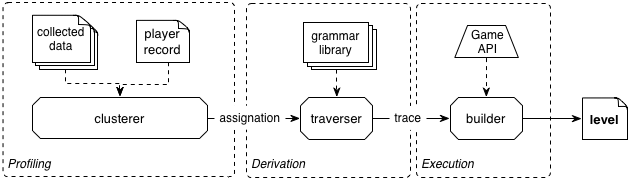
\includegraphics[width=1.5\columnwidth]{layers.png}}
\caption{Layers and modules of the proposed architecture}
\label{layers}
\end{figure*}

The architecture presented in this paper is related to that idea, albeit with some new modifications. The classification, for instance, is not a process based on heuristics, but data-driven from records of players. After an assignation has been made, this results in the selection of a set of rules; they affect not only the frequency of elements as in the above model, but also their placement adjacent to each other. This is done to enforce level aesthetics as envisioned by the designer and improve the sense of order.



\section{Overview}

The proposed architecture can be seen in Figure~\ref{layers}. It is composed of three layers:

\begin{itemize}
	
\item \textbf{Profiling}: identifies the user and sets a series of parameters to define his profile

\item \textbf{Derivation}: uses the parameters obtained in the first layer to create a plan to build the level

\item \textbf{Execution}: the third executes that plan to produce the actual level as output

\end{itemize}

The three layers are briefly introduced below, as a first approach to their content.

\subsection{Profiling}

In the first layer, the system ascertains the characteristics of the player. The conclusions reached here will guide the rest of the modules down the correct path. For this reason, it was decided to employ a clustering process. Clustering means that players will be defined by the parameters than make them stand out from the rest, that is, the features that make them special. This allows to focus on those characteristics to tailor the experience to their tastes. The fact that a player enjoys a particular part of a stage may or may not be a remarkable event for customization, depending on how often players find that part likable.

Once a player has been assigned to a cluster, this assignment is passed down to the second layer.

\subsection{Derivation}

The second layer uses the assignment from the first layer to make a ``plan'' for building the level. Different players will be assigned different plans, and, furthermore, the same player should not be assigned the same plan twice. The chosen method will have to have some inherent randomess.

Levels in platform games can be seen as a succession of repeated basic symbols. For example, in the \textit{Mario} series, some of those symbols might be a gap to jump over, a pipe with an enemy, or a row of blocks. Moreover, the symbols follow some logic in the placement, based on what comes before. Two pipes are never placed immediately adjacent after another, for instance.

Since it became apparent that levels had their own language, it was decided to express their structure as a grammar. The derivation rules act as possible branches to take when building the level, and the symbols of the grammar, the level pieces (called \textit{chunks}) to place on it. Each player cluster from the top layer is linked to a grammar, called \textit{schematic}, expressing what chunks can be put together -- and how often -- in that playstyle. 

The schematic is converted to an automaton and traversed, picking the transitions by the weight that their corresponding rule have in the grammar. A list of nodes (a \textit{trace}) is output by this process.

\subsection{Execution}

Finally the trace is interpreted by the execution layer. Each item on the list produces a call to the game API. This layer converts the plan made by the automaton into an actual playable level, by relying on the level building functions of framework. It's the final intermediary between the architecture proposed here and the game.

In the next sections we'll explore the different layers more in detail, then at the end we'll review the results obtained upon their application.





\section{Profiling}
\label{overviewprofiling}

This first step of the system is intended to ``get to know'' the user to control the rest of the process in the right direction. The goals for this layer are to differentiate the player by finding his characteristic playstyle, without the need of asking him, since sometimes, user input can be misleading. For example, when polling the players on their proficiency, newcomer players are known to badly estimate their skills \cite{dunningkruger,skilled,overestimate}.

So it was decided to use records for a clustering process. This would classify the players on how they fare in the playstyle spectrum compared to others, and the system can focus on the differential aspects for their personalization. The Mario AI Championship platform stores two kinds of user records: global metrics from each game run, and a detailed log of the actions taken. Since the effort is to evaluate the player on his overall style instead of analyzing specific timestamped events, it was decided to use only the aggregated metrics, where parameters on time, enemy kills, deaths, coins and blocks are kept. Table~\ref{parameters} shows a listing of those metrics.


\begin{table*}[ht]
\begin{center}
\renewcommand{\arraystretch}{1.3}
\caption{Parameters recorded by the Mario AI Platform}
\label{parameters}
\begin{tabular}{|c|c|c|}
\hline
\textit{ArmoredTurtlesKilled} & \textit{CannonBallKilled} & \textit{ChompFlowersKilled} \\
\hline
GoombasKilled & \textit{GreenTurtlesKilled} & \textit{JumpFlowersKilled} \\
\hline
\textit{RedTurtlesKilled} & aimlessJumps & coinBlocksDestroyed \\
\hline
coinsCollected & completionTime & duckNumber \\
\hline
emptyBlocksDestroyed & enemyKillByFire & \textit{enemyKillByKickingShell} \\
\hline
jumpsNumber & \textit{kickedShells} & percentageBlocksDestroyed \\
\hline
percentageCoinBlocksDestroyed & percentageEmptyBlockesDestroyed & percentagePowerBlockDestroyed \\
\hline
powerBlocksDestroyed & timeRunningLeft & timeRunningRight \\
\hline
timeSpentDucking & timeSpentRunning & \textit{timesOfDeathByArmoredTurtle} \\
\hline
\textit{timesOfDeathByCannonBall} & \textit{timesOfDeathByChompFlower} & \textit{timesOfDeathByFallingIntoGap} \\
\hline
timesOfDeathByGoomba & \textit{timesOfDeathByGreenTurtle} & \textit{timesOfDeathByJumpFlower} \\
\hline
\textit{timesOfDeathByRedTurtle} & timesPressedRun & timesSwichingPower \\
\hline
totalCoinBlocks & totalCoins & totalEmptyBlocks \\
\hline
totalEnemies & totalTime & totalTimeFireMode \\
\hline
totalTimeLargeMode & totalTimeLittleMode & totalpowerBlocks \\
\hline
\end{tabular}
\end{center}
\end{table*}


Since the clusters are made to discern playing styles, the records have to be collected from presenting the players with comparable challenges. Two players playing one a hard level and another an easy one will produce great disparity in their records, even if their playstyle is quite similar. It was chosen to use the default random levels provided by the Mario AI Championship platform. They are quite simple levels, approachable for beginners but enjoyable by experts.

The clustering was performed trying to find three specific clusters, identified already in previous works on the field (see work by G. Jacobs and G Takahashi in \cite{mario2010}). In bold, the nicknames given to the them in this paper:

\begin{itemize}
	
	\item \textbf{speeders}, focused in the main goal (traversing the level) and caring very little for other aspects
	
	\item \textbf{explorers}, playing the game in no hurry, interacting with every item and walking down every path available
	
	\item and \textbf{intermediates}, that hold a position in between
	
\end{itemize}

These profiles can be thought as a spectrum ranging from quick rush to slow walk, from simple play to extensive interaction. Equivalents can be drawn to similar spectrums in other games. For example, in the card game \textit{Magic: the Gathering}, the two main strategies for winning are \textit{aggro}, consisting in quickly overwhelming the opponents with simple creatures; and \textit{control}, that slowly builds dominion over the game until dealing the final blow\footnote{A third common strategy, \textit{combo}, exploits peculiarities in the interaction between some elements of the game to win the match instantly. This is, however, a unique strategy exclusive to \textit{Magic}. }. Other archetypes like \textit{midrange} or \textit{aggro-control} lie somewhere in the middle. \cite{magicdecks}

To find those three clusters, it was decided to rely on the Weka \footnote{\url{http://www.cs.waikato.ac.nz/~ml/weka/}} library for the process. It is a powerful, proved library that offers a wide range of clustering algorithms. As a metric to compare their performance, the value of their log likelihood was chosen, which is a popular paramter for this purpose. Log likelihood, however, can't be calculated for non-density-based algorithms (like \textit{EM}), so the other algorithms tried, \textit{FarthestFirst}, \textit{HierarchicalClusterer}, \textit{sIB}, \textit{XMeans}, and \textit{SimpleKMeans} have to be wrapped in Weka's \textit{MakeDensityBasedCluster} to provide this value. These algorithms were chosen because they can be told to look for a specific number of clusters, as it was intended.

Finally, this process has the advantage of being able to be run offline, that is, previous to the actual level generation. Once the clusters are found in the sampled data, the results can be stored, and accessed just when a new player comes. It is at that moment when they are read, the player assigned to one of those clusters, and the assignation passed down to the next layer.




\section{Derivation}
\label{derivation}

When we assign the player to a cluster, we implicitly assign him a grammar, per its cluster. Those grammars, called \textit{schematics}, define the structure of a level using a syntax similar to Backus-Naur Form. Figure~\ref{minigrammar} shows an example of a reduced schematic.

\begin{figure}[htp]
	\begin{lstlisting}
initial = hub ;

hub = flat hub , 0.3
		| pipe hub , 0.4
		| coins hub , 0.3;

flat = FLAT ;

pipe = PIPE ;

coins = COINS , 0.8
		| COINS coins , 0.2;
	\end{lstlisting}
\caption{A small sample schematic}
\label{minigrammar}
\end{figure}

Tokens in uppercase are terminal symbols; tokens in lowercase are nonterminals. The numbers at the end of rules are weights (no number means default weight). The schematics explain how to build a level; a rule with a bigger weight has more probabilities of being chosen. Schematics are written by hand by the designers, although the terminals are predefined by the execution layer (see section \ref{execution}) and depend on the level building parts offered by the game API (called \textit{chunks}). For example, in the example schematic from figure~\ref{minigrammar} the terminals are \textbf{PIPE}, \textbf{COINS} and \textbf{FLAT}, representing the production of a pipe, a coin and some flat ground.

Grammars defined in schematics are context-free, and cycle on their right (that is, the nonterminals on the left of a derivation chain are always expanded first and resolve to terminals). Going back to the schematic on figure~\ref{minigrammar}, from the start symbol we go to \textbf{hub} and then can derive \textbf{pipe hub}, \textbf{coins hub} or \textbf{flat hub}. The choice would be random, albeit conditioned by the weights of the rules. \textbf{pipe} would resolve to \textbf{PIPE} (a pipe), \textbf{coins} to a small loop \textbf{COINS} (two coins), and \textbf{flat} to \textbf{FLAT} (a strip of flat ground). Then, \textbf{hub} would go back to the ``branchìng hub'' and the process will be repeated. The reason for having a neverending cycle is that schematics are designed to be infinite, so levels of any length can be produced. Derivation is stopped whe the desired level size is reached.

As it was said, each cluster determines what schematic is picked, as it has derivations and weights tailored to the needs of its corresponding profile (but same available set of terminals, although it may decide not to use some of them). To read the schematics, the parse2 library\footnote{\url{http://www.parse2.com/}} was used to convert schematics into Java objects, that in turn became automata by creating a weighted directed graph. Symbols are turned into states and derivation rules into weighted transitions (links between states).

Traversing the automaton is alike to create the derivation tree. From the top node, or rule, a transition is chosen giving bigger odds to those with bigger weights. Terminal [states] are added to the trace, nonterminal [states] are pushed to a temporary stack. Then the top element of the stack is popped, and the process repeated until stopped. Figures~\ref{minitrace} shows a sample trace from the schematic in figure~\ref{minigrammar} after ten iterations:

\begin{figure}[htp]
	\begin{lstlisting}
FLAT
PIPE
FLAT
COINS
COINS
FLAT
COINS
COINS
PIPE
PIPE
	\end{lstlisting}
\caption{Sample trace for the simple schematic}
\label{minitrace}
\end{figure}

Because schematics have rules that expand towards their right, that means the tree is traversed depth-first. The resulting trace will be the basis for later construction of the level, since it uniquely identifies the parts that would have to be placed in it, and in what order. More accurately, it defines the ``actions`'' that will have to be called by the execution layer. It's like a plan for building the level. Two equal traces define the same level.


\section{Execution}
\label{execution}

The final part of the system is to take the trace produced in the derivation layer, and execute the plan in it. Each terminal or \textit{gene} in it represents a call to a level-building function. Those functions were written as wrappers over the game API, and produce a small part of the level, a \textit{chunk}.

For convenience, all chunks were made to be two blocks length. As long as all chunks were the same size:

\begin{itemize}

	\item traces of equal length produced levels of equal length

	\item and conversedly, levels of equal size had traces of equal length, so

	\item the number of genes in the trace for a level of a given length could be predicted

\end{itemize}

The actual size was not important, although since schematics offer a way to control macrostructure (big picture design), having more chunks, but smaller, meant more control on microstructure (small picture design). One block was to small, since pipes occupy two, and one-block gaps are never found in Mario games.

The reason behind separating the trace and actual level building is threefold. First, it allows for visual or gameplay changes to happen through all levels thanks to the decoupling of symbol and functionality. For example, coins could be removed from the game at once by simply changing the parsing of the gene \textbf{COIN} from calling the coin chunk function to the flat ground chunk function. Secondly, it allows the level to be produced independently of the framework, so it can be reinterpreted by being processed on another API. And finally, it provides a method for identifying levels; they can be compared, analyzed or stored in a library as their trace.


\section{Results}

Testing of the system required data from user play to detect the clusters. To collect the player records, social networks like Twitter\footnote{\url{http://twitter.com}}, Facebook\footnote{\url{http://facebook.com}} and Reddit\footnote{\url{http://reddit.com}}, and word of mouth, were used to encourage participation in this research.

Users were directed to a webpage\footnote{\url{http://diz.es/mario/}} where they were instructed to download a package. It was a zip file, with a copy of the platform as provided by the competition organization (no modifications) and easy instructions to follow. Scripts were made for every major platform (Windows, OSX, Linux) so the process of playing was reduced to double clicking a file. After that, participants were instructed to mail back the text files that had been generated after the game (the log records). No indications about the goals for the game where given except to ``play normally'' to have fun and not worry about completing the level or waiting until practice made you better.

At the time of this article, 118 different player records had been received. Before analyzing them, some parameters were filtered in preprocessing. The default random level generation algorithm of the Mario AI Championship platform does not create gaps or enemies other than goombas. Parameters related to interaction with those elements were therefore always zero in the records, and thus they were excluded from the study. In Table~\ref{parameters}, in section~\ref{overviewprofiling}, those elements were marked in \textit{italics}.

	\begin{table}
	\begin{center}
	\renewcommand{\arraystretch}{1.3}
	\caption{Log Likelihood of the different cluster algorithms}
	\label{loglikelihood}
	\begin{tabular}{|c|c|}
	\hline
	EM & -81.14 \\
	\hline
	SimpleKMeans & -82.67 \\
	\hline
	XMeans & -82.99 \\
	\hline
	sIB & -83.86 \\
	\hline
	Cobweb & -85.02 \\
	\hline
	FarthestFirst & -86.44 \\
	\hline
	HierarchicalClusterer & -87.63 \\
	\hline
	\end{tabular}
	\end{center}
	\end{table}

The data was then fed to Weka, where the available clusteirng algorithms were tested. As shown in Table~\ref{loglikelihood}, the best results, as per the log likelihood value that is common to employ in these cases, was obtained by the Expectation-Maximization algorithm. Not only that, but the clusters represented the three profiles looked for (speeders, exploreres and intermediates). As a sample, in Table~\ref{averages} some parameters are shown where clear differences in averages between the clusters were found. Additionally, Figure~\ref{timeRunningLeft} shows the timeSpentRunningLeft metric plotted against cluster assignation.


\begin{table}
\begin{center}
\renewcommand{\arraystretch}{1.3}
\caption{Averages of the clusters for some sample parameters }
\label{averages}
\begin{tabular}{|l|r|r|r|}
\hline

\textbf{Parameters} & \textbf{speeders} & \textbf{intermediates} & \textbf{explorers} \\

\hline

\textit{GoombasKilled} & & & \\
  mean &                              2.0901   & 5.8411   &  7.366 \\
  std. dev. &                          1.6154  &  3.1408   & 3.6322 \\

\hline

\textit{coinsCollected} & & & \\
  mean   &                            30.7347  & 42.1388  & 69.4287 \\
  std. dev.  &                        15.4715  &  14.011  & 19.7648 \\

\hline

\textit{emptyBlocksDestroyed} & & & \\
  mean        &                        0.9315  & 12.1945  & 18.7678 \\
  std. dev.    &                       1.5705  &  7.3109  & 12.8681 \\

\hline

\textit{jumpsNumber} & & & \\
  mean             &                  49.1143  & 81.8984  & 146.6187 \\
  std. dev.        &                  16.6757  & 14.7733  & 34.2822 \\

\hline

\textit{timeRunningLeft} & & & \\
  mean              &                 11.1026  & 28.2323  & 57.7755 \\
  std. dev.         &                  8.4517   & 9.5608  & 20.8693 \\

\hline

\textit{timeSpentRunning} & & & \\
  mean                      &          28.053  & 17.5453  & 12.7792 \\
  std. dev.             &             29.2726  & 25.0467  & 11.4864 \\

\hline

\textit{totalTime} & & & \\
  mean                  &            103.2858  & 161.713  & 323.7268 \\
  std. dev.            &              49.5377  & 31.2944  & 76.2367 \\

\hline

\end{tabular}
\end{center}
\end{table}

\begin{figure}[htp]
\centerline{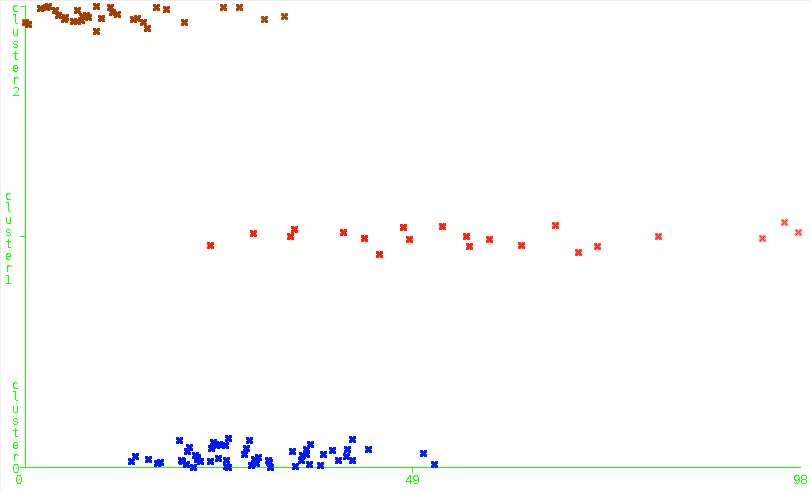
\includegraphics[width=0.9\columnwidth]{timeRunningLeft.png}}
\label{timeRunningLeft}
\caption{The data points for timeRunningLeft. Time is on the horizontal axis, and clusters are on the vertical axis. Speeders on top, explorers on the middle, and intermediates on the bottom.}
\end{figure}

For each of those clusters, a grammar was written per the methodology in section \ref{derivation}. Figure~\ref{speedersch} shows the rules associated to the \textit{speeder} profile. Notice must be taken on how all branches sprouting from the \textbf{hub} end in some flat ground, as spacing between elements. Cluttered screens seemed to impact as messy and unfocused. Also remarkable is the low probability for gaps with stairs, since they were found to be frustrating for those players as they break the flow of running. It is also lacking double rows of blocks, that were severely disregarded by speeders as well.

\begin{figure*}[htp]
	\begin{lstlisting}
initial			= hub ;

flat			= FLAT hub ;

hub				= coins flat, 17
				| pipe flat , 12
				| blocks flat , 20
				| enemies flat , 20
				| cannon flat , 8
				| gaps flat , 19;
		
flat 			= FLAT flat, 5
				| FLAT hub , 95;

coins 			= COINS , 80
				| COINS coins , 20;

pipe 			= PIPE 
				| PIPEPIRANHA ;
		
blocks			= singleblock , 20
				| singleblock blocks , 80 ;
		
singleblock		= BLOCKPOWERUP
				| BLOCKCOINS , 10
				| BLOCKEMPTY , 50 ;
		
enemies			= singlenemy , 20
				| singlenemy enemies , 80 ;
				
singlenemy		= GOOMBA , 10
				| REDTURTLE , 3
				| GREENTURTLE , 3
				| SPIKY ;
				
cannon			= CANNON ;

gaps			= GAP , 5
				| STAIRSUP GAP STAIRSDOWN ;

	\end{lstlisting}
\caption{The speeder schematic}
\label{speedersch}
\end{figure*}

A sample run through the automaton built from this grammar can be seen in the sample trace in figure~\ref{speedertrace}, and a screenshot from the stage built from that trace in figure~\ref{screenshot}.

\begin{figure}[htp]
	\begin{lstlisting}
	...
	BLOCKPOWERUP
	BLOCKPOWERUP
	GAP
	FLAT
	COINS
	COINS
	GOOMBA
	GOOMBA
	...
	\end{lstlisting}
\caption{Sample of a trace built from the speeder schematic}
\label{speedertrace}
\end{figure}

\begin{figure}[htp]
\centerline{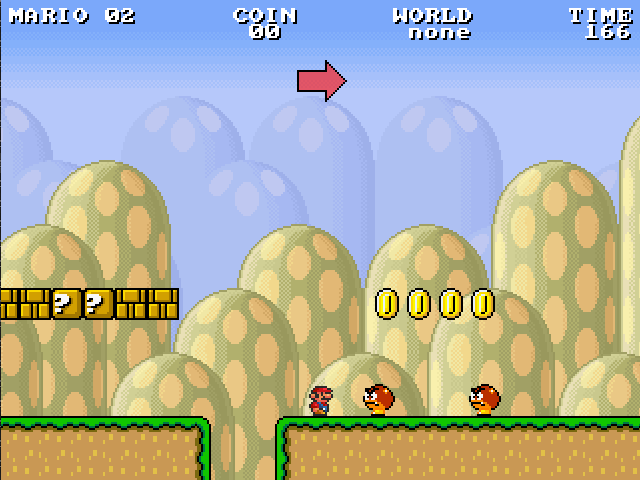
\includegraphics[width=0.9\columnwidth]{screenshot.png}}
\label{screenshot}
\caption{Sample level built from the speeders schematic}
\end{figure}

\section{Conclusions}

The architecture for adaptive procedural level generation presented here combines clustering for player identification with grammars for level structure definition. The separation of functionality means that the parameters guiding the process are not intermixed with the actual generation process and either of those two parts may be swapped out for another approach.

Use of grammars results in a random, yet ordered way of producing levels. New possibilities can be added to a level just by creating rules that combine the available chunks in different ways or with different frequencies. At the same time, having different grammars for each profile means diverse necessities and styles can be catered for while not disturbing other players for whom the changes are not meant.

By defining a unique trace for each level as output of the derivation process, before its execution into a playable level itself, an easy, unequivocal way of storing levels for later reference has been developed. Levels can now be compared, mixed or measured against other metrics by statistical analysis on its components.  

\subsection*{Future work}

We hope to refine this methodology by group control evaluation, further tuning the grammar derivations and frequencies. We also hope to explore the possibilities that the trace opens for genetic combination of levels, guided perhaps by percentages of profiling obtained by fuzzy clustering (that is, each player has a degree of belonging to a cluster, instead of being all-or-nothing). Another option, using the same profiling technique, would be to use those percentages to pick between derivation rules of different grammars.

\section*{Acknowledgments}
This work has been supported by the
Spanish Ministry of Science and Innovation under grant
TIN2010-19872 (ABANT).

% Trigger a \newpage just before a given reference number in order to
% balance the columns on the last page.  Adjust the value as needed;
% it may need to be readjusted if the document is modified later.
%\IEEEtriggeratref{8}
% The "triggered" command can be changed if desired:
%\IEEEtriggercmd{\enlargethispage{-5in}}

% The references section can either be generated by hand or by an
% automatic tool like BibTeX.  If using BibTex, use the standard IEEEtran
% bibliography style.
\bibliographystyle{IEEEtran.bst}
%
% The argument to \bibliography is/are the name(s) of your BibTeX file(s)
% that contains string definitions and bibliography database(s).
\bibliography{IEEEabrv,jorgedizpico}
%
% If you generate the bibliography by hand, or if you copy in the
% resultant .bbl file, set the second argument of \begin to the number of
% references in the bibliography (used to reserve space for the reference
% number labels box).

%\begin{thebibliography}{3}
%\bibitem{book}
%A.~Great, \emph{This is the book title}.\hskip 1em plus 0.5em minus 0.4em\relax
%  This is the name of the publisher, 2006.

%\bibitem{conf}
%F.~Author, S.~Author, and T.~NonRelatedAuthor, ``This is the paper title,'' in
%  \emph{This is the proceedings title}, 2008, pp. 1--8.

%\bibitem{article}
%B.~Myself, ``This is the title of the journal article,'' \emph{This is the name
%  of the journal}, pp. 1--30, 2007.
%\end{thebibliography}

% That's all folks...
\end{document}
